\documentclass[a4paper, 14pt]{extarticle}
\usepackage{float}
% Поля
%--------------------------------------
\usepackage{geometry}
\geometry{a4paper,tmargin=2cm,bmargin=2cm,lmargin=3cm,rmargin=1cm}
%--------------------------------------


%Russian-specific packages
%--------------------------------------
\usepackage[T2A]{fontenc}
\usepackage[utf8]{inputenc} 
\usepackage[english, main=russian]{babel}
%--------------------------------------

\usepackage{textcomp}

% Красная строка
%--------------------------------------
\usepackage{indentfirst}               
%--------------------------------------             


%Graphics
%--------------------------------------
\usepackage{graphicx}
\graphicspath{ {./images/} }
\usepackage{wrapfig}
%--------------------------------------

% Полуторный интервал
%--------------------------------------
\linespread{1.3}                    
%--------------------------------------

%Выравнивание и переносы
%--------------------------------------
% Избавляемся от переполнений
\sloppy
% Запрещаем разрыв страницы после первой строки абзаца
\clubpenalty=10000
% Запрещаем разрыв страницы после последней строки абзаца
\widowpenalty=10000
%--------------------------------------

%Списки
\usepackage{enumitem}

%Подписи
\usepackage{caption} 

%Гиперссылки
\usepackage{hyperref}

\hypersetup {
	unicode=true
}

%Рисунки
%--------------------------------------
\DeclareCaptionLabelSeparator*{emdash}{~--- }
\captionsetup[figure]{labelsep=emdash,font=onehalfspacing,position=bottom}
%--------------------------------------

\usepackage{tempora}

%Листинги
%--------------------------------------
\usepackage{listings}
\lstset{
  basicstyle=\ttfamily\footnotesize, 
  %basicstyle=\footnotesize\AnkaCoder,        % the size of the fonts that are used for the code
  breakatwhitespace=false,        % sets if automatic breaks shoulbd only happen at whitespace
  breaklines=true,                 % sets automatic line breaking
  captionpos=t,                    % sets the caption-position to bottom
  inputencoding=utf8,
  frame=single,                    % adds a frame around the code
  keepspaces=true,                 % keeps spaces in text, useful for keeping indentation of code (possibly needs columns=flexible)
  keywordstyle=\bf,       % keyword style
  numbers=left,                    % where to put the line-numbers; possible values are (none, left, right)
  numbersep=5pt,                   % how far the line-numbers are from the code
  xleftmargin=25pt,
  xrightmargin=25pt,
  showspaces=false,                % show spaces everywhere adding particular underscores; it overrides 'showstringspaces'
  showstringspaces=false,          % underline spaces within strings only
  showtabs=false,                  % show tabs within strings adding particular underscores
  stepnumber=1,                    % the step between two line-numbers. If it's 1, each line will be numbered
  tabsize=2,                       % sets default tabsize to 8 spaces
  title=\lstname                   % show the filename of files included with \lstinputlisting; also try caption instead of title
}
%--------------------------------------

%%% Математические пакеты %%%
%--------------------------------------
\usepackage{amsthm,amsfonts,amsmath,amssymb,amscd}  % Математические дополнения от AMS
\usepackage{mathtools}                              % Добавляет окружение multlined
\usepackage[perpage]{footmisc}
%--------------------------------------

%--------------------------------------
%			НАЧАЛО ДОКУМЕНТА
%--------------------------------------

\begin{document}

%--------------------------------------
%			ТИТУЛЬНЫЙ ЛИСТ
%--------------------------------------
\begin{titlepage}
\thispagestyle{empty}
\newpage


%Шапка титульного листа
%--------------------------------------
\vspace*{-60pt}
\hspace{-65pt}
\begin{minipage}{0.3\textwidth}
\hspace*{-20pt}\centering

\includegraphics[width=\textwidth]{emblem}
\end{minipage}
\begin{minipage}{0.67\textwidth}\small \textbf{
\vspace*{-0.7ex}
\hspace*{-6pt}\centerline{Министерство науки и высшего образования Российской Федерации}
\vspace*{-0.7ex}
\centerline{Федеральное государственное бюджетное образовательное учреждение }
\vspace*{-0.7ex}
\centerline{высшего образования}
\vspace*{-0.7ex}
\centerline{<<Московский государственный технический университет}
\vspace*{-0.7ex}
\centerline{имени Н.Э. Баумана}
\vspace*{-0.7ex}
\centerline{(национальный исследовательский университет)>>}
\vspace*{-0.7ex}
\centerline{(МГТУ им. Н.Э. Баумана)}}
\end{minipage}
%--------------------------------------

%Полосы
%--------------------------------------
\vspace{-25pt}
\hspace{-35pt}\rule{\textwidth}{2.3pt}

\vspace*{-20.3pt}
\hspace{-35pt}\rule{\textwidth}{0.4pt}
%--------------------------------------

\vspace{1.5ex}
\hspace{-35pt} \noindent \small ФАКУЛЬТЕТ\hspace{80pt} <<Информатика и системы управления>>

\vspace*{-16pt}
\hspace{47pt}\rule{0.83\textwidth}{0.4pt}

\vspace{0.5ex}
\hspace{-35pt} \noindent \small КАФЕДРА\hspace{50pt} <<Теоретическая информатика и компьютерные технологии>>

\vspace*{-16pt}
\hspace{30pt}\rule{0.866\textwidth}{0.4pt}
  
\vspace{11em}

\begin{center}
\Large {\bf Летучка № 1 } \\ 
\large {\bf по курсу <<Разработка мобильных приложений>>} \\
\large <<Мобильное приложение управления двумя переменными>> 
\end{center}\normalsize

\vspace{8em}


\begin{flushright}
  {Студент группы ИУ9-71Б Баев Д.А \hspace*{15pt}\\ 
  \vspace{2ex}
  Преподаватель Посевин Д. П.\hspace*{15pt}}
\end{flushright}

\bigskip

\vfill
 

\begin{center}
\textsl{Москва 2023}
\end{center}
\end{titlepage}
%--------------------------------------
%		КОНЕЦ ТИТУЛЬНОГО ЛИСТА
%--------------------------------------

\renewcommand{\ttdefault}{pcr}

\setlength{\tabcolsep}{3pt}
\newpage
\setcounter{page}{2}

\section{Задание}\label{Sect::task}
1. Реализовать мобильное приложение управления двумя переменными на сайте ioControl.ru

2. Для выполнения задачи использовать пакет 'http/dart'.
\newpage
\section{Исходный код}

Исходный код программы представлен в листинге~\ref{lst:code1}

\begin{figure}[H]
\begin{lstlisting}[language={},caption={Реализация мобильного приложения},label={lst:code1}]
import 'dart:html';

import 'package:flutter/material.dart';
import 'package:http/http.dart' as http;

void main() {
  runApp(const MyApp());
}

class MyApp extends StatelessWidget {
  const MyApp({super.key});

  // This widget is the root of your application.
  @override
  Widget build(BuildContext context) {
    return MaterialApp(
      title: 'Flutter Demo',
      theme: ThemeData(
        colorScheme: ColorScheme.fromSeed(seedColor: Colors.deepPurple),
        useMaterial3: true,
      ),
      home: const MyHomePage(title: 'Flutter Demo Home Page'),
    );
  }
}

class MyHomePage extends StatefulWidget {
  const MyHomePage({super.key, required this.title});
  final String title;

  @override
  State<MyHomePage> createState() => _MyHomePageState();
}

class _MyHomePageState extends State<MyHomePage> {
  int _counter = 0;

  void _incrementCounter() {
    setState(() {
      _counter++;
    });
  }

  void _getLampRequestON() { 
    setState(() {
      http.get(Uri.parse('http://iocontrol.ru/api/sendData/Fly_mobile/Lamp/1')).then((response) {
        print("Response status: ${response.statusCode}");
        print("Response body: ${response.body}");
      }).catchError((error){
        print("Error: $error");
      });
    });
  }
  void _getLampRequestOFF() {
    // <----- Step 2
    setState(() {
      http.get(Uri.parse('http://iocontrol.ru/api/sendData/Fly_mobile/Lamp/0'))
          .then((response) {
        print("Response status: ${response.statusCode}");
        print("Response body: ${response.body}");
      }).catchError((error) {
        print("Error: $error");
      });
    });
  }
    void _getDoorRequestOFF() {
      // <----- Step 2
      setState(() {
        http.get(
            Uri.parse('http://iocontrol.ru/api/sendData/Fly_mobile/Door/0'))
            .then((response) {
          print("Response status: ${response.statusCode}");
          print("Response body: ${response.body}");
        }).catchError((error) {
          print("Error: $error");
        });
      });
    }
  void _getDoorRequestON() {
    // <----- Step 2
    setState(() {
      http.get(
          Uri.parse('http://iocontrol.ru/api/sendData/Fly_mobile/Door/1'))
          .then((response) {
        print("Response status: ${response.statusCode}");
        print("Response body: ${response.body}");
      }).catchError((error) {
        print("Error: $error");
      });
    });
  }
  @override
  Widget build(BuildContext context) {
    return Scaffold(
      appBar: AppBar(
        title: Text(widget.title),
      ),
      body: Center(
          mainAxisAlignment: MainAxisAlignment.center,
          children: <Widget>[
            const Text(
              'You have pushed the button this many times:',
            ),
            Text(
              '$_counter',
              style: Theme.of(context).textTheme.headlineMedium,
            ),
            TextButton(
              style: ButtonStyle(
                foregroundColor: MaterialStateProperty.all<Color>(Colors.blue),
              ),
              onPressed: _getLampRequestON,
              child: Text('ON_LAMP'),
            ),
            TextButton( 
              style: ButtonStyle(
                foregroundColor: MaterialStateProperty.all<Color>(Colors.blue),
              ),
              onPressed: _getLampRequestOFF,
              child: Text('OFF_LAMP'),
            ),
            TextButton(
              style: ButtonStyle(
                foregroundColor: MaterialStateProperty.all<Color>(Colors.blue),
              ),
              onPressed: _getDoorRequestON,
              child: Text('ON_DOOR'),
            ),
            TextButton( 
              style: ButtonStyle(
                foregroundColor: MaterialStateProperty.all<Color>(Colors.blue),
              ),
              onPressed: _getDoorRequestOFF,
              child: Text('OFF_DOOR'),
            )
          ],
        ),
      ),
      floatingActionButton: FloatingActionButton(
        onPressed: _incrementCounter,
        tooltip: 'Increment',
        child: const Icon(Icons.add),
      ), // This trailing comma makes auto-formatting nicer for build methods.
    );

  }
}

\end{lstlisting}
\end{figure}


\section{Результаты}

Результат приведен на рисунке~\ref{fig:img1}

\begin{figure}[H]
\centering
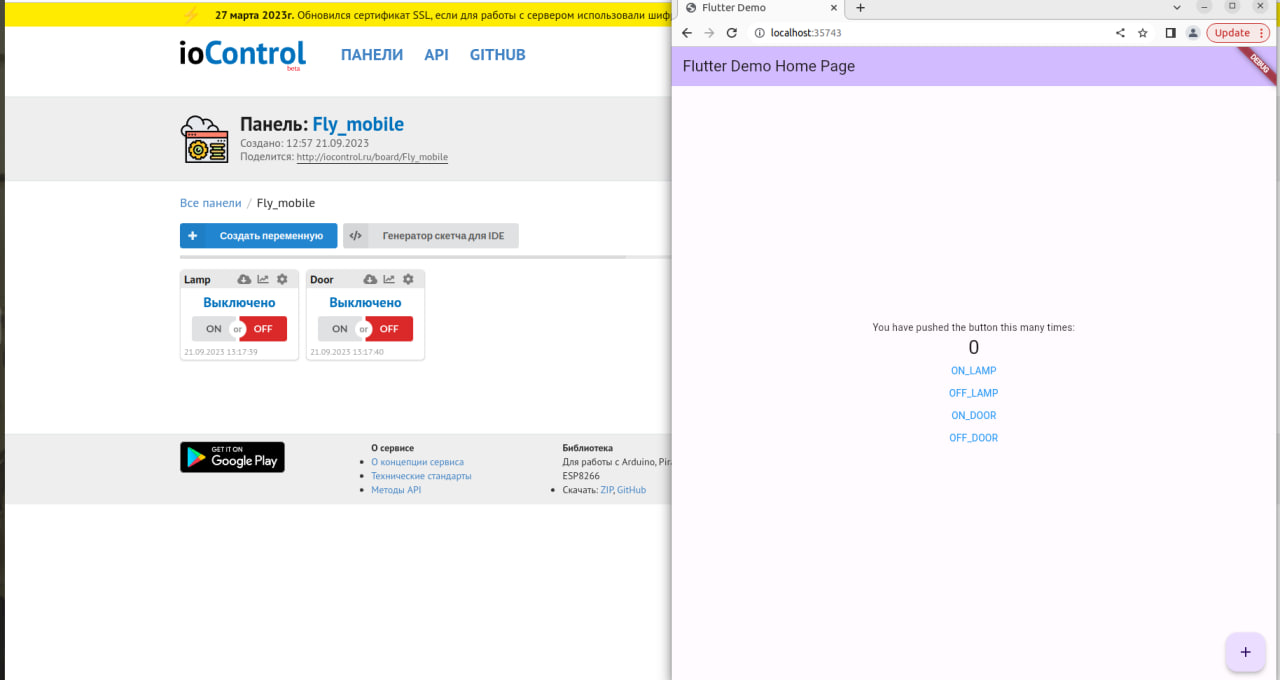
\includegraphics[width=0.8\textwidth]{images/res1.jpg}
\caption{Результат работы мобильного приложения}
\label{fig:img1}
\end{figure}



\section{Выводы}
В рамках данной летучки был разработан макет мобильного приложения на flutter, который позволяет взаимодействовать с интернетом вещей, например передавать лампочке запросы на включение-выключение.
\end{document}
